%!TeX program = xelatex
\documentclass[12pt,hyperref,a4paper,UTF8]{ctexart}
\usepackage{BUAAReport}
\usepackage{listings}
\usepackage{xcolor}
\usepackage{booktabs}
\usepackage{array}
\usepackage{caption}
\usepackage{setspace}
\setstretch{1.5}
\usepackage{enumitem}
\setlist[itemize]{itemsep=0pt, parsep=0pt}
\usepackage{pgfplots}
\pgfplotsset{compat=1.18}
\usepackage{tikz}
\usepackage{amsmath}
\usepackage{float}
\usepackage{graphicx}
\usepackage{subcaption}
\usepackage{fancyhdr}

\setmainfont{Times New Roman}
\setlength{\headheight}{14pt}

\fancypagestyle{mainstyle}{
  \fancyhf{}
  \fancyhead[C]{\small 基于 MindSpore 的 TorchDrug 论文复现}
  \fancyfoot[C]{\thepage}
  \renewcommand{\headrulewidth}{0.4pt}
  \renewcommand{\footrulewidth}{0pt}
}

\fancypagestyle{plain}{
  \fancyhf{}
  \fancyhead[C]{\small 基于 MindSpore 的 TorchDrug 论文复现}
  \fancyfoot[C]{\thepage}
  \renewcommand{\headrulewidth}{0.4pt}
  \renewcommand{\footrulewidth}{0pt}
}

% 代码样式设置
\lstset{
  basicstyle=\ttfamily\small,
  keywordstyle=\color{blue}\bfseries,
  commentstyle=\color{gray},
  stringstyle=\color{red!70!black},
  numbers=left,
  numberstyle=\tiny\color{gray},
  stepnumber=1,
  breaklines=true,
  frame=single,
  tabsize=4,
  showstringspaces=false,
  language=C++
}

%封面页设置
%封面页设置
{   
    %标题
    \title{ 
        \vspace{1.5cm}
        \heiti \Huge \textbf{{AI框架与科学计算课程大作业报告}} \par
        \vspace{1cm} 
        \heiti \Large {\underline{基于 MindSpore 的 TorchDrug 论文复现}}
        \vspace{1cm}
    }

    \author{
        \vspace{0.7cm}
        \kaishu\Large 学院\ \dlmu[9cm]{计算机学院} \\ %学院
        \vspace{0.7cm}
        \kaishu\Large 专业\ \dlmu[9cm]{计算机技术} \\ %学院
        \vspace{0.7cm}
        \kaishu\Large 姓名\ \dlmu[9cm]{卢静颖、应素文} \\ %班级
        \vspace{0.7cm}
        \kaishu\Large 学号\ \dlmu[9cm]{ZY2506214、ZY2506132} \qquad \\ %姓名 
    }
    \vspace{2cm}
    \date{\today} % 默认为今天的日期，可以注释掉不显示日期
}

\begin{document}

\cover
\thispagestyle{empty}

\newpage
\tableofcontents
\thispagestyle{empty}

\newpage
\setcounter{page}{1}
\pagestyle{mainstyle}
\thispagestyle{mainstyle}

\section{小组基础信息}

\begin{table}[H]
  \centering
  \caption{课程大作业基础信息}
  \begin{tabular}{@{}>{\bfseries}p{0.22\textwidth}p{0.70\textwidth}@{}}
    \toprule
    项目 & 内容\\
    \midrule
    小组队名 & 分子图学习复现小组\\
    小组成员 & \textbf{卢静颖}，ZY2506214；应素文，ZY2506132\\
    科学任务 & 使用图神经网络进行药物虚拟筛选中的分子活性二分类预测\\
    论文标题 & TorchDrug: A Powerful and Flexible Machine Learning Platform for Drug Discovery\\
    科学领域 & 生物医药、药物发现、分子机器学习、图神经网络\\
    复现框架 & MindSpore。实验对照使用 TorchDrug，但复现训练代码不直接调用 PyTorch 或 TorchDrug 训练模块。\\
    \bottomrule
  \end{tabular}
\end{table}

\section{背景介绍}

药物发现是人工智能与生命科学交叉领域中极具代表性的科学计算问题。一个新药从靶点发现到临床应用通常需要经历候选分子筛选、先导化合物优化、体外实验、动物实验以及多期临床试验等环节，研发周期长、实验成本高、失败风险大。传统高通量筛选需要在实验室中对大量化合物进行逐一测试，虽然能够获得可靠的活性数据，但面对数以百万计甚至数以亿计的候选分子空间时，实验资源很难覆盖全部候选。因此，在真实实验之前利用机器学习模型对候选分子的活性、毒性和药代动力学性质进行预测，已经成为现代计算药物发现中的重要技术路线。

分子具有天然的图结构。原子可以看作图中的节点，化学键可以看作图中的边，原子类型、价态、手性、芳香性、杂化方式、环信息以及化学键类型等化学信息都可以转化为节点或边特征。与传统分子指纹和人工描述符相比，图神经网络可以直接在分子拓扑结构上进行消息传递，不需要将分子强行压缩为固定规则的人工特征。对于药物虚拟筛选任务而言，这种表示方式具有直观的化学意义：模型可以从局部官能团、环结构和原子连接关系中学习与生物活性相关的结构模式，再通过图级 readout 得到整个分子的表示。

本次课程大作业选择复现论文 \emph{TorchDrug: A Powerful and Flexible Machine Learning Platform for Drug Discovery}\cite{torchdrug}。该论文提出了一个面向药物发现任务的机器学习平台 TorchDrug，试图解决药物发现研究中数据集接口不统一、模型复用困难、任务封装重复、评估流程难以对齐等问题。TorchDrug 将分子性质预测、分子生成、逆合成预测、蛋白质任务和知识图谱推理等药物发现任务纳入统一框架，使研究者能够较方便地组合数据、模型、任务和训练引擎。

由于课程要求必须使用 MindSpore 深度学习框架，不能直接使用 PyTorch 或 TorchDrug 的训练代码，本项目并不复现完整 TorchDrug 平台，而是选取论文中最基础也最典型的分子性质预测任务作为复现目标。具体而言，本项目使用 RDKit 从 SMILES 字符串构造分子图，参考 TorchDrug 的默认原子与化学键特征，使用 MindSpore 实现 GIN 与 GAT 两类图神经网络，并在 BACE 和 HIV 两个公开数据集上完成分子活性二分类预测。通过该任务可以展示 TorchDrug 论文中“统一图表示、统一模型接口、统一训练评估流程”的核心思想，也能检验这些思想迁移到 MindSpore 框架时的实现难点。

\section{问题定义}

分子活性预测可以形式化为图级二分类问题。给定一个 SMILES 字符串 $s$，首先使用 RDKit 将其解析为分子图：
\[
G=(V,E),
\]
其中 $V=\{v_1,v_2,\ldots,v_n\}$ 表示原子集合，$E\subseteq V\times V$ 表示化学键集合。对于每个原子 $v_i$，构造节点特征向量 $\mathbf{x}_i$；对于每条化学键 $(i,j)$，构造边特征向量 $\mathbf{e}_{ij}$。节点特征主要描述原子本身的化学属性，边特征主要描述化学键类型和立体信息。

模型需要学习一个从分子图到二分类 logit 的映射：
\[
f_{\theta}(G)=z,\quad z\in\mathrm{R}.
\]
其中 $\theta$ 为模型参数，$z$ 经过 sigmoid 函数后得到分子属于活性类别的概率：
\[
\hat{p}=\sigma(z)=\frac{1}{1+\exp(-z)}.
\]
对于 BACE 数据集，标签 $y\in\{0,1\}$ 表示分子是否为 BACE-1 抑制剂；对于 HIV 数据集，标签表示分子是否具有抑制 HIV replication 的活性。训练目标是最小化二元交叉熵损失：
\[
\mathcal{L}
=-\frac{1}{N}\sum_{i=1}^{N}
\left[y_i\log\sigma(z_i)+(1-y_i)\log(1-\sigma(z_i))\right].
\]
实际实现中采用 MindSpore 的 \texttt{BCEWithLogitsLoss}，该损失函数将 sigmoid 与交叉熵合并计算，能够避免显式 sigmoid 在极大或极小 logit 上产生的数值不稳定。

评价指标采用 AUROC 和 AUPRC。AUROC 衡量模型将正样本排在负样本前面的整体能力；AUPRC 衡量 precision-recall 曲线下的面积，对正负样本不均衡任务更加敏感。HIV 数据集中活性分子比例较低，如果只看准确率容易掩盖模型对少数正类的识别能力，因此 AUPRC 是本任务中非常重要的指标。由于 AUROC 和 AUPRC 只依赖预测分数的排序，本项目在评估时直接使用模型输出 logits 作为排序分数，以尽量贴近 TorchDrug 的指标计算方式。

\section{研究现状}

早期分子性质预测通常依赖人工设计的分子描述符或分子指纹，例如分子量、氢键供受体数量、LogP、拓扑极性表面积、Morgan fingerprint 等。这些特征具有较强的化学解释性，并且可以与随机森林、支持向量机、梯度提升树等传统机器学习模型结合，在许多小规模任务上取得稳定表现。然而，人工特征通常依赖专家知识，且很难完整表达分子图的拓扑结构和高阶相互作用。当任务涉及复杂官能团组合、长程依赖或结构相似但活性差异明显的分子时，固定指纹的表达能力会受到限制。

MoleculeNet\cite{moleculenet} 的提出推动了分子机器学习任务的标准化。该工作整理了多个公开分子数据集，将分子性质预测划分为量子化学、物理化学、生物活性和毒性等不同类别，并提出一套较统一的数据划分和评价指标。BACE 和 HIV 都是 MoleculeNet 中常用的二分类基准数据集。MoleculeNet 的重要意义在于，它使不同模型能够在相对统一的数据和指标下进行比较，也暴露出分子机器学习面临的数据稀缺、类别不平衡、分布外泛化和 scaffold split 泛化等挑战。

图神经网络的发展为分子性质预测提供了更加自然的建模方式。Message Passing Neural Network（MPNN）\cite{mpnn} 将多种分子图模型统一为消息传递框架：每一层中节点从邻居接收消息，再更新自身表示，最终通过 readout 得到图级表示。该框架非常适合分子图，因为原子周围的化学环境可以通过多层消息传递逐步扩大感受野。GIN\cite{gin} 从图同构判别能力出发分析图神经网络表达能力，指出求和聚合加 MLP 的结构在理论上具有较强区分能力，因此常用于图分类任务。GAT\cite{gat} 则引入注意力机制，为不同邻居分配不同权重，使模型能够学习哪些相邻原子或键对当前节点表示更重要。

在药物发现应用中，Yang 等\cite{dmpnn} 系统分析了学习型分子表示在性质预测中的表现，并提出 directed message passing neural network，在多个公开与工业数据集上取得较好结果。这类研究说明，图神经网络不仅能作为学术基准模型，也具有辅助真实药物研发流程的潜力。但是，不同研究往往使用不同的数据预处理、划分方式、超参数和评估脚本，导致结果复现较困难。TorchDrug\cite{torchdrug} 正是在这一背景下提出的平台型工作。它提供统一的数据集、图结构、模型、任务和训练引擎，降低了药物发现机器学习实验的工程复杂度。

MindSpore 是面向端边云场景的深度学习框架，支持自动微分、动态图和静态图等能力。使用 MindSpore 复现 TorchDrug 的分子性质预测任务，一方面符合课程对 AI 学习框架的要求，另一方面也可以观察同一科学任务在不同深度学习框架中的实现差异。本项目选择 GIN 和 GAT 作为复现模型，是因为二者分别代表了强表达能力的求和聚合模型和基于注意力的邻居加权模型，能够覆盖 TorchDrug 中常见的图神经网络范式。

\section{论文方法}

TorchDrug 论文的核心贡献是提出一个面向药物发现的灵活机器学习平台，而不是只提出单一模型。平台将药物发现任务抽象为若干可组合模块，包括数据集、图表示、模型、任务、训练引擎和指标评估。论文中的平台结构如图~\ref{fig:torchdrug-architecture} 所示：最上层的 \texttt{torchdrug.core.Engine} 负责训练、评估、模型保存与配置读取；中间的 \texttt{torchdrug.tasks} 将分子性质预测、预训练分子表示、分子设计、逆合成预测和知识图谱推理等科学任务封装为统一接口；底层的 \texttt{torchdrug.data}、\texttt{torchdrug.datasets} 和 \texttt{torchdrug.transforms} 负责图、分子、数据集与数据变换；\texttt{torchdrug.layers} 和 \texttt{torchdrug.models} 则提供卷积、池化、readout、GCN、GAT、MPNN 等可复用模型组件。

\begin{figure}[H]
  \centering
  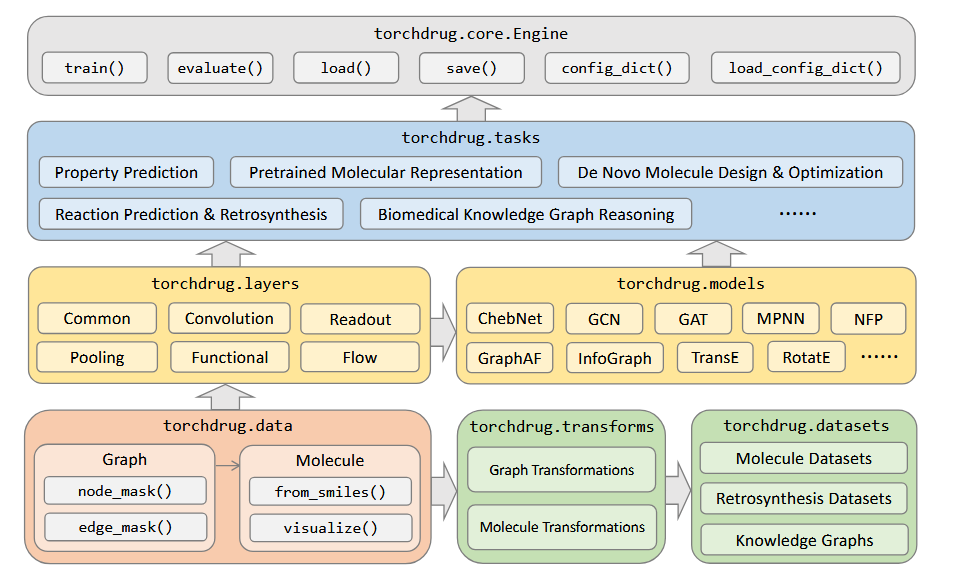
\includegraphics[width=0.92\textwidth]{figures/torchdrug.png}
  \caption{TorchDrug 论文中的平台架构示意图}
  \label{fig:torchdrug-architecture}
\end{figure}

结合图~\ref{fig:torchdrug-architecture} 可以看出，TorchDrug 的方法并不是将某一个 GNN 模型孤立地用于药物发现，而是把“数据读取—图结构表示—模型编码—任务损失—训练评估”组织成统一流水线。对于本项目关注的分子性质预测任务，实际运行路径可以理解为：首先由数据集模块读取 BACE 或 HIV 中的 SMILES 和活性标签；随后由分子图构造模块调用 RDKit 将 SMILES 转换为 \texttt{Molecule}/\texttt{Graph} 表示；再由图神经网络模型对节点、边和图级表示进行编码；最后由性质预测任务计算二分类损失，并输出 AUROC、AUPRC 等指标。该过程在 TorchDrug 中由 PyTorch 生态实现，本项目则按照相同任务抽象在 MindSpore 中重新实现核心训练流程。为了说明本项目的复现落点，图~\ref{fig:pipeline} 给出了简化后的分子性质预测流程。

\begin{figure}[H]
  \centering
  \begin{tikzpicture}[
    node distance=1.6cm,
    every node/.style={font=\small},
    box/.style={draw, rounded corners, align=center, minimum width=2.5cm, minimum height=0.9cm},
    arrow/.style={->, thick}
  ]
    \node[box] (smiles) {SMILES\\分子字符串};
    \node[box, right of=smiles, xshift=2.1cm] (rdkit) {RDKit\\分子图构造};
    \node[box, right of=rdkit, xshift=2.1cm] (feature) {原子/键\\特征编码};
    \node[box, below of=feature] (gnn) {GIN/GAT\\图神经网络};
    \node[box, left of=gnn, xshift=-2.1cm] (readout) {Sum Readout\\图级表示};
    \node[box, left of=readout, xshift=-2.1cm] (pred) {MLP/Linear\\活性预测};
    \draw[arrow] (smiles) -- (rdkit);
    \draw[arrow] (rdkit) -- (feature);
    \draw[arrow] (feature) -- (gnn);
    \draw[arrow] (gnn) -- (readout);
    \draw[arrow] (readout) -- (pred);
  \end{tikzpicture}
  \caption{本项目复现的分子性质预测流程}
  \label{fig:pipeline}
\end{figure}

在图表示方面，TorchDrug 将原子作为节点，将化学键作为边。节点特征包括原子符号、手性、度数、形式电荷、氢原子数量、自由基电子数、杂化方式、芳香性以及是否在环中等信息；边特征包括键类型、键方向、立体构型以及是否共轭。本项目参考 TorchDrug 默认特征集合，在 MindSpore 项目中使用 RDKit 实现相同思想的特征提取。由于课程任务关注分子二分类，图级标签由 CSV 中的 \texttt{Class} 或 \texttt{HIV\_active} 字段提供。

在模型方面，GIN 的基本思想是对邻居节点表示进行求和，并使用 MLP 更新节点表示。第 $k$ 层节点 $v$ 的更新可以写为：
\[
\mathbf{h}_{v}^{(k)}
=\mathrm{MLP}^{(k)}
\left((1+\epsilon)\mathbf{h}_{v}^{(k-1)}
+\sum_{u\in\mathcal{N}(v)}
\left(\mathbf{h}_{u}^{(k-1)}+\phi_e(\mathbf{e}_{uv})\right)\right),
\]
其中 $\phi_e$ 是边特征线性映射。相比均值聚合，求和聚合保留了邻居数量信息，通常具有更强的图结构区分能力。本项目使用 MindSpore 的 gather 和 unsorted segment sum 完成消息收集与聚合，并在 torchdrug-like 变体中加入 BatchNorm、shortcut、concat hidden 和 sum readout。

GAT 的思想是对不同邻居赋予不同注意力权重。对边 $(u,v)$，模型根据源节点、目标节点和边特征计算 attention score，再在同一目标节点的入边上做归一化：
\[
\alpha_{uv}=\frac{\exp(a_{uv})}{\sum_{u'\in\mathcal{N}(v)}\exp(a_{u'v})}.
\]
为了避免 $\exp$ 溢出，本项目参考 TorchDrug 的实现方式，在指数运算前对同一目标节点的 score 减去 segment max。这样不会改变 softmax 结果，却能显著提升数值稳定性。GAT 的优势在于能够让模型自动学习不同化学邻居的重要性，但代价是计算量和数值敏感性都高于 GIN。

\section{复现实现}

本项目核心文件包括：\texttt{dataset.py} 负责数据下载、CSV 读取、SMILES 解析、scaffold/random split 和 batch 拼接；\texttt{features.py} 负责原子与化学键特征；\texttt{models.py} 负责 MindSpore 版本的 GIN/GAT；\texttt{trainer.py} 负责损失函数、优化器、训练循环和评估；\texttt{run\_experiment.py} 提供命令行入口。整个训练过程使用 MindSpore，未直接调用 PyTorch 或 TorchDrug 的训练代码。

为了使实验协议与 TorchDrug 更一致，本项目对实现进行了三项关键对齐。第一，BACE 默认使用与 TorchDrug \texttt{ordered\_scaffold\_split} 兼容的划分方式，不再随机打乱同一 scaffold 内部样本。第二，将主要超参数统一为 hidden dim 256、GNN 层数 4、训练 100 轮；HIV 数据集规模较大，实际实验中 batch size 使用 512 以提高训练效率。第三，结果记录采用 \texttt{best\_valid\_auroc} 策略，即保存验证集 AUROC 最优轮次对应的测试集指标，并在结果 CSV 中记录 \texttt{selected\_epoch}。

\begin{lstlisting}[language=Python, caption={TorchDrug ordered scaffold split 对齐实现片段}]
def scaffold_split(dataset, seed, fractions=(0.8, 0.1, 0.1)):
    scaffold_to_indices = defaultdict(list)
    for index, smiles in enumerate(dataset.smiles):
        scaffold = MurckoScaffold.MurckoScaffoldSmiles(
            smiles=smiles, includeChirality=True)
        scaffold_to_indices[scaffold].append(index)

    scaffold_sets = [
        sorted(scaffold_set)
        for _, scaffold_set in sorted(
            scaffold_to_indices.items(),
            key=lambda item: (len(item[1]), sorted(item[1])[0]),
            reverse=True)
    ]
\end{lstlisting}

\begin{lstlisting}[language=Python, caption={MindSpore GAT attention 稳定化实现片段}]
score = self.reduce_sum(key * ops.expand_dims(self.query, 0), -1)
score = ops.maximum(score, score * self.negative_slope)
score = score - self.segment.gather_rows(
    self.segment.max(score, node_out, num_node), node_out)

exp_score = ops.exp(score)
normalizer = self.segment.sum(exp_score, node_out, num_node)
attention = exp_score / (
    self.segment.gather_rows(normalizer, node_out) + self.eps)
\end{lstlisting}

训练循环使用 MindSpore 自动微分接口 \texttt{value\_and\_grad}。每个 batch 中，所有分子的节点和边被拼接为一个大图，并使用 \texttt{node2graph} 标识节点所属分子。模型输出 shape 为 batch size $\times 1$ 的 logits，随后使用 \texttt{BCEWithLogitsLoss} 计算二分类损失。评估阶段不再进行梯度计算，收集验证集或测试集所有 logits 后计算 AUROC 和 AUPRC。

\section{实验设置}

实验数据来自公开 MoleculeNet/DeepChem CSV。BACE 用于预测分子是否为 BACE-1 抑制剂，标签字段为 \texttt{Class}；HIV 用于预测分子是否具有抑制 HIV replication 的活性，标签字段为 \texttt{HIV\_active}。表~\ref{tab:dataset} 总结了数据集设置。

\begin{table}[H]
  \centering
  \caption{数据集与任务设置}
  \label{tab:dataset}
  \begin{tabular}{@{}p{0.10\textwidth}p{0.12\textwidth}p{0.14\textwidth}p{0.16\textwidth}p{0.38\textwidth}@{}}
    \toprule
    数据集 & 任务 & 划分方式 & 标签字段 & 说明\\
    \midrule
    BACE & 二分类 & scaffold & Class & 预测分子是否为 BACE-1 抑制剂，数据规模较小，scaffold split 对泛化评估影响明显。\\
    HIV & 二分类 & random & HIV\_active & 预测分子是否具有抑制 HIV replication 活性，样本量较大且类别不均衡。\\
    \bottomrule
  \end{tabular}
\end{table}

\begin{table}[H]
  \centering
  \caption{复现实验超参数}
  \label{tab:hyper}
  \begin{tabular}{l c c c c c c}
    \toprule
    数据集 & 模型 & hidden dim & 层数 & batch size & epoch & 结果选择\\
    \midrule
    BACE & GIN/GAT & 256 & 4 & 256 & 100 & best valid AUROC\\
    HIV  & GIN/GAT & 256 & 4 & 512 & 100 & best valid AUROC\\
    \bottomrule
  \end{tabular}
\end{table}

核心运行命令如下：
\begin{lstlisting}[language=bash, caption={MindSpore 四组核心实验命令}]
python run_experiment.py --dataset bace --model gin --epoch 100 --batch_size 256 --seed 0 --device_target GPU --selection best_valid_auroc
python run_experiment.py --dataset bace --model gat --epoch 100 --batch_size 256 --seed 0 --device_target GPU --selection best_valid_auroc
python run_experiment.py --dataset hiv --model gin --epoch 100 --batch_size 512 --seed 0 --split random --device_target GPU --selection best_valid_auroc
python run_experiment.py --dataset hiv --model gat --epoch 100 --batch_size 512 --seed 0 --split random --device_target GPU --selection best_valid_auroc
\end{lstlisting}

\section{复现结果}

\subsection{MindSpore 复现结果}

表~\ref{tab:ms-result} 给出了 MindSpore 框架下四组核心实验结果。所有结果均记录验证集 AUROC 最优轮次对应的测试集表现。

\begin{table}[H]
  \centering
  \caption{MindSpore 框架下的复现实验结果}
  \label{tab:ms-result}
  \resizebox{\textwidth}{!}{%
  \begin{tabular}{l l c c c c c}
    \toprule
    数据集 & 模型 & 最优轮次 & Valid AUROC & Valid AUPRC & Test AUROC & Test AUPRC\\
    \midrule
    BACE & GIN & 81 & 0.7751 & 0.9584 & 0.7103 & 0.7174\\
    BACE & GAT & 82 & 0.7099 & 0.9349 & 0.7507 & 0.7449\\
    HIV  & GIN & 70 & 0.8566 & 0.4811 & 0.7886 & 0.3747\\
    HIV  & GAT & 66 & 0.8591 & 0.4918 & 0.7704 & 0.3776\\
    \bottomrule
  \end{tabular}
  }
\end{table}

\subsection{TorchDrug 对照结果}

为分析复现效果，使用 TorchDrug 框架在相同数据集和相近超参数下运行对照实验，结果如表~\ref{tab:td-result} 所示。

\begin{table}[H]
  \centering
  \caption{TorchDrug 框架下的对照实验结果}
  \label{tab:td-result}
  \resizebox{\textwidth}{!}{%
  \begin{tabular}{l l c c c c c}
    \toprule
    数据集 & 模型 & Epoch & Valid AUROC & Valid AUPRC & Test AUROC & Test AUPRC\\
    \midrule
    BACE & GIN & 100 & 0.8593 & 0.8157 & 0.8017 & 0.8304\\
    BACE & GAT & 100 & 0.7835 & 0.7424 & 0.8095 & 0.8340\\
    HIV  & GIN & 100 & 0.7755 & 0.3314 & 0.8234 & 0.3652\\
    HIV  & GAT & 100 & 0.7904 & 0.3391 & 0.8348 & 0.3738\\
    \bottomrule
  \end{tabular}
  }
\end{table}

\begin{table}[H]
  \centering
  \caption{MindSpore 与 TorchDrug 测试集结果差值（MindSpore - TorchDrug）}
  \label{tab:diff}
  \begin{tabular}{l l c c}
    \toprule
    数据集 & 模型 & Test AUROC 差值 & Test AUPRC 差值\\
    \midrule
    BACE & GIN & -0.0913 & -0.1130\\
    BACE & GAT & -0.0588 & -0.0891\\
    HIV  & GIN & -0.0348 & +0.0095\\
    HIV  & GAT & -0.0644 & +0.0039\\
    \bottomrule
  \end{tabular}
\end{table}

\begin{figure}[H]
  \centering
  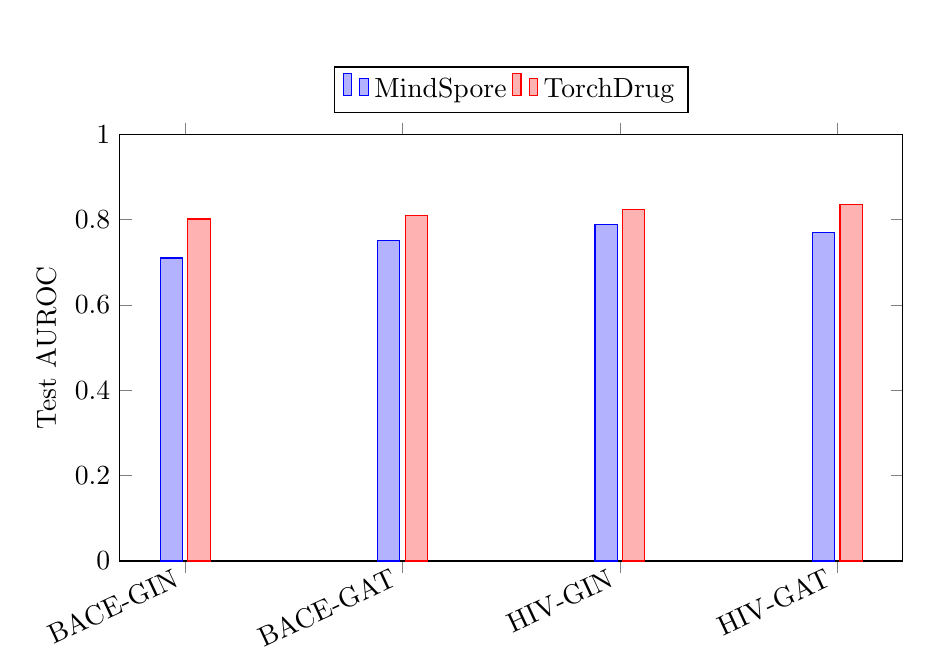
\begin{tikzpicture}
    \begin{axis}[
      ybar,
      ymin=0,
      ymax=1,
      width=0.95\textwidth,
      height=7cm,
      bar width=8pt,
      ylabel={Test AUROC},
      symbolic x coords={BACE-GIN,BACE-GAT,HIV-GIN,HIV-GAT},
      xtick=data,
      x tick label style={rotate=25,anchor=east},
      legend style={at={(0.5,1.05)},anchor=south,legend columns=2}
    ]
      \addplot coordinates {(BACE-GIN,0.7103) (BACE-GAT,0.7507) (HIV-GIN,0.7886) (HIV-GAT,0.7704)};
      \addplot coordinates {(BACE-GIN,0.8017) (BACE-GAT,0.8095) (HIV-GIN,0.8234) (HIV-GAT,0.8348)};
      \legend{MindSpore,TorchDrug}
    \end{axis}
  \end{tikzpicture}
  \caption{MindSpore 与 TorchDrug 测试集 AUROC 对比}
  \label{fig:auroc}
\end{figure}

\begin{figure}[H]
  \centering
  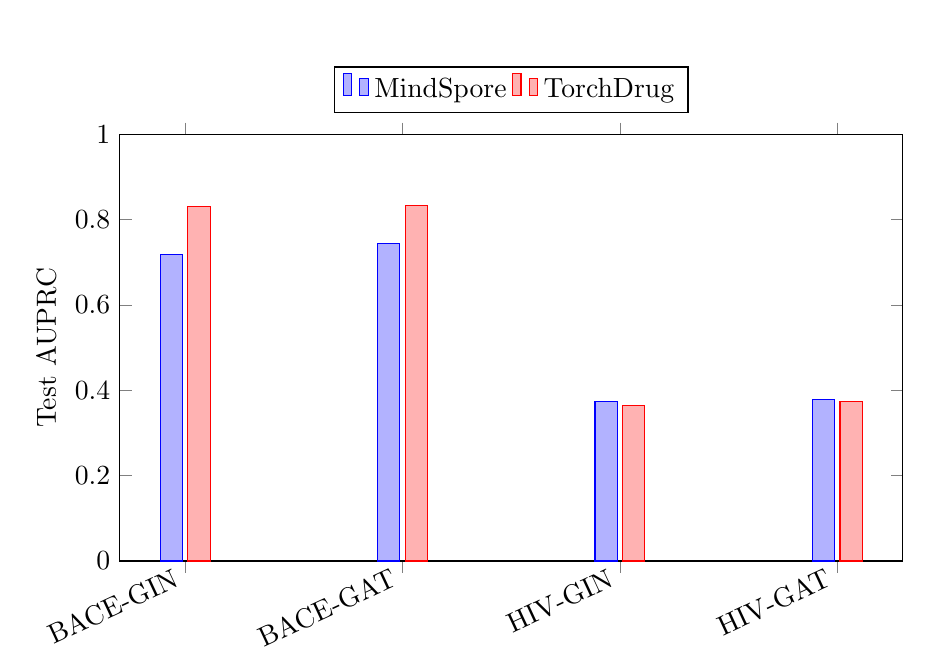
\begin{tikzpicture}
    \begin{axis}[
      ybar,
      ymin=0,
      ymax=1,
      width=0.95\textwidth,
      height=7cm,
      bar width=8pt,
      ylabel={Test AUPRC},
      symbolic x coords={BACE-GIN,BACE-GAT,HIV-GIN,HIV-GAT},
      xtick=data,
      x tick label style={rotate=25,anchor=east},
      legend style={at={(0.5,1.05)},anchor=south,legend columns=2}
    ]
      \addplot coordinates {(BACE-GIN,0.7174) (BACE-GAT,0.7449) (HIV-GIN,0.3747) (HIV-GAT,0.3776)};
      \addplot coordinates {(BACE-GIN,0.8304) (BACE-GAT,0.8340) (HIV-GIN,0.3652) (HIV-GAT,0.3738)};
      \legend{MindSpore,TorchDrug}
    \end{axis}
  \end{tikzpicture}
  \caption{MindSpore 与 TorchDrug 测试集 AUPRC 对比}
  \label{fig:auprc}
\end{figure}

\section{结果分析}

从 BACE 数据集结果看，MindSpore 版本的 GAT 在测试集上优于 MindSpore 版本的 GIN，Test AUROC 从 0.7103 提升到 0.7507，Test AUPRC 从 0.7174 提升到 0.7449。这说明在当前 scaffold split 下，注意力机制对 BACE 测试集具有一定帮助。不过与 TorchDrug 对照相比，MindSpore 版本的 BACE 测试指标仍然偏低。GIN 的 Test AUROC 低 0.0913，Test AUPRC 低 0.1130；GAT 的 Test AUROC 低 0.0588，Test AUPRC 低 0.0891。BACE 数据规模较小，scaffold split 后验证集和测试集样本数量有限，少量分子的排序变化就会对 AUROC 和 AUPRC 造成明显影响，因此该数据集上的指标波动较大。

从 HIV 数据集结果看，MindSpore 版本的测试 AUROC 低于 TorchDrug 对照，但测试 AUPRC 与 TorchDrug 接近。MindSpore GIN 的 Test AUPRC 为 0.3747，高于 TorchDrug GIN 的 0.3652；MindSpore GAT 的 Test AUPRC 为 0.3776，也略高于 TorchDrug GAT 的 0.3738。由于 HIV 是类别不均衡任务，AUPRC 对正类检索质量更加敏感，因此这一结果说明 MindSpore 复现模型在活性分子检索能力上达到了接近 TorchDrug 的水平。

MindSpore 与 TorchDrug 结果不完全一致是可以预期的。首先，本项目是教学型简化复现，虽然对齐了 ordered scaffold split、edge-list 图表示、默认特征和 best valid AUROC 结果选择，但底层算子、初始化、BatchNorm 行为、优化器实现和数据加载方式仍与 PyTorch/TorchDrug 存在差异。其次，GAT 对数值稳定性更敏感，本项目通过 segment max 稳定化避免 attention 溢出，但 scatter mean/sum 的精确行为仍可能与 TorchDrug 不完全一致。最后，本项目没有进行大规模超参数搜索，也没有使用预训练模型，因此结果不能理解为完整平台性能复现，而应理解为对 TorchDrug 分子性质预测核心流程的 MindSpore 复现。

从课程目标角度看，本项目完成了三个层面的工作。第一，在科学任务层面，项目将药物虚拟筛选抽象为分子图二分类任务，并给出了明确的数学定义。第二，在框架实现层面，项目没有直接调用 TorchDrug 训练代码，而是使用 MindSpore 自行实现 GIN、GAT、loss、优化器调用和训练评估循环。第三，在实验验证层面，项目在 BACE 和 HIV 两个数据集上得到了可复现的 AUROC/AUPRC 结果，并与 TorchDrug 框架结果进行了对照分析。

\section{局限性与改进方向}

本项目仍然存在一些局限。首先，复现范围只覆盖了 TorchDrug 论文中的分子性质预测任务，没有覆盖分子生成、逆合成预测、蛋白质结构任务和知识图谱推理等更复杂模块。因此，本项目更准确地说是对 TorchDrug 核心思想的任务级复现，而不是完整平台复现。其次，当前训练效率低于 TorchDrug 原版，尤其在 HIV 大数据集和 GAT 模型上更加明显。这与 MindSpore 动态图模式、Python 端 batch 拼接、缺少专门的 scatter 图算子优化等因素有关。再次，实验只使用单个随机种子，虽然已经记录了 seed 和 selected epoch，但仍不足以全面反映模型稳定性。

后续可以从以下方向改进。第一，增加多随机种子实验，报告均值和标准差，减少单次运行偶然性的影响。第二，进一步对齐 TorchDrug 的 GAT 聚合细节，包括 scatter mean、attention 归一化和参数初始化。第三，尝试 MindSpore 静态图模式或自定义高效图算子，降低 HIV 数据集上的训练耗时。第四，将实验扩展到 BBBP、ClinTox、Tox21 等更多 MoleculeNet 数据集，以获得更全面的复现结论。第五，在报告展示层面，可以加入训练曲线、混淆矩阵或 PR 曲线，进一步分析模型在正负样本上的具体表现。

\section{结论}

本项目围绕 TorchDrug 论文中的分子性质预测任务，使用 MindSpore 实现了一个简化但完整的药物虚拟筛选流程。项目从 SMILES 出发，使用 RDKit 构造分子图，参考 TorchDrug 默认特征构造节点和边特征，采用 edge-list 形式组织 batch，并实现了 GIN 与 GAT 两种图神经网络模型。训练过程使用 MindSpore 的 \texttt{BCEWithLogitsLoss} 和 \texttt{Adam}，评估指标为 AUROC 与 AUPRC。

实验结果表明，MindSpore 版本能够成功完成 BACE 和 HIV 分子活性二分类预测任务。在 BACE 上，MindSpore GAT 优于 MindSpore GIN，但整体低于 TorchDrug 对照；在 HIV 上，MindSpore 版本的测试 AUPRC 与 TorchDrug 接近，说明其对活性分子的检索能力具有一定有效性。综合来看，本项目验证了 TorchDrug 论文中“统一数据处理、图模型、任务封装和指标评估”的核心思想可以迁移到 MindSpore 框架中，也体现了不同深度学习框架和底层图算子实现对复现结果的影响。

\begin{thebibliography}{99}

\bibitem{torchdrug}
Zhu Z, Shi C, Zhang Z, Liu S, Xu M, Yuan X, Zhang Y, Chen J, Cai H, Lu J, et al. TorchDrug: A Powerful and Flexible Machine Learning Platform for Drug Discovery[EB/OL]. arXiv:2202.08320, 2022. \url{https://arxiv.org/abs/2202.08320}.

\bibitem{moleculenet}
Wu Z, Ramsundar B, Feinberg E N, Gomes J, Geniesse C, Pappu A S, Leswing K, Pande V. MoleculeNet: a benchmark for molecular machine learning[J]. Chemical Science, 2018, 9: 513--530.

\bibitem{gin}
Xu K, Hu W, Leskovec J, Jegelka S. How Powerful are Graph Neural Networks?[C]//International Conference on Learning Representations. 2019.

\bibitem{gat}
Veličković P, Cucurull G, Casanova A, Romero A, Liò P, Bengio Y. Graph Attention Networks[C]//International Conference on Learning Representations. 2018.

\bibitem{mpnn}
Gilmer J, Schoenholz S S, Riley P F, Vinyals O, Dahl G E. Neural Message Passing for Quantum Chemistry[C]//International Conference on Machine Learning. 2017.

\bibitem{dmpnn}
Yang K, Swanson K, Jin W, Coley C, Eiden P, Gao H, et al. Analyzing Learned Molecular Representations for Property Prediction[J]. Journal of Chemical Information and Modeling, 2019, 59(8): 3370--3388.

\bibitem{rdkit}
RDKit: Open-source cheminformatics software[EB/OL]. \url{https://www.rdkit.org/}.

\end{thebibliography}

\end{document}
